\documentclass{article}

% if you need to pass options to natbib, use, e.g.:
\PassOptionsToPackage{numbers, compress}{natbib}
% before loading neurips_2025

% The authors should use one of these tracks.
% Before accepting by the NeurIPS conference, select one of the options below.
% 0. "default" for submission
%\usepackage{neurips_2025}
% the "default" option is equal to the "main" option, which is used for the Main Track with double-blind reviewing.
% 1. "main" option is used for the Main Track
%  \usepackage[main]{neurips_2025}
% 2. "position" option is used for the Position Paper Track
%  \usepackage[position]{neurips_2025}
% 3. "dandb" option is used for the Datasets & Benchmarks Track
 % \usepackage[dandb]{neurips_2025}
% 4. "creativeai" option is used for the Creative AI Track
%  \usepackage[creativeai]{neurips_2025}
% 5. "sglblindworkshop" option is used for the Workshop with single-blind reviewing
 % \usepackage[sglblindworkshop]{neurips_2025}
% 6. "dblblindworkshop" option is used for the Workshop with double-blind reviewing
%\usepackage[dblblindworkshop]{neurips_2025_ml4ps}

% After being accepted, the authors should add "final" behind the track to compile a camera-ready version.
% 1. Main Track
 % \usepackage[main, final]{neurips_2025}
% 2. Position Paper Track
%  \usepackage[position, final]{neurips_2025}
% 3. Datasets & Benchmarks Track
 % \usepackage[dandb, final]{neurips_2025}
% 4. Creative AI Track
%  \usepackage[creativeai, final]{neurips_2025}
% 5. Workshop with single-blind reviewing
%  \usepackage[sglblindworkshop, final]{neurips_2025}
% 6. Workshop with double-blind reviewing
\usepackage[final]{neurips_2025_ml4ps}
% Note. For the workshop paper template, both \title{} and \workshoptitle{} are required, with the former indicating the paper title shown in the title and the latter indicating the workshop title displayed in the footnote.
% For workshops (5., 6.), the authors should add the name of the workshop, "\workshoptitle" command is used to set the workshop title.
%\workshoptitle{Machine Learning and the Physical Sciences}

% "preprint" option is used for arXiv or other preprint submissions
 % \usepackage[preprint]{neurips_2025}

% to avoid loading the natbib package, add option nonatbib:
%\usepackage[nonatbib]{neurips_2025}

\usepackage[utf8]{inputenc} % allow utf-8 input
\usepackage[T1]{fontenc}    % use 8-bit T1 fonts
\usepackage{hyperref}       % hyperlinks
\usepackage{url}            % simple URL typesetting
\usepackage{booktabs}       % professional-quality tables
\usepackage{amsfonts}       % blackboard math symbols
\usepackage{nicefrac}       % compact symbols for 1/2, etc.
\usepackage{microtype}      % microtypography
\usepackage{xcolor}         % colors
\usepackage{amsmath}
\usepackage{graphicx}
\usepackage{float}          % custom float for the algorithm (no external algo pkg needed)
\newfloat{algorithm}{!ht}{loa}
\floatname{algorithm}{Algorithm}

% Define a simple inline comment command
\newcommand{\inlinerui}[1]{\textcolor{blue}{\textbf{[Rui: #1]}}}
% Note. For the workshop paper template, both \title{} and \workshoptitle{} are required, with the former indicating the paper title shown in the title and the latter indicating the workshop title displayed in the footnote.
\title{PALM: Physics-Aware Leakage Minimizer}

% The \author macro works with any number of authors. There are two commands
% used to separate the names and addresses of multiple authors: \And and \AND.
%
% Using \And between authors leaves it to LaTeX to determine where to break the
% lines. Using \AND forces a line break at that point. So, if LaTeX puts 3 of 4
% authors names on the first line, and the last on the second line, try using
% \AND instead of \And before the third author name.

\author{%
  Rodrigo Ferreira\\
  Pritzker School of Molecular Engineering\\
  University of Chicago\\
  Chicago, IL, USA \\
  \texttt{rpferreira@uchicago.edu} \\
  % examples of more authors
  \And
  Ray Zhu\\
  Pritzker School of Molecular Engineering\\
  University of Chicago\\
  Chicago, IL, USA \\
  \texttt{rzhu16@uchicago.edu} \\
  \And
  Rui Ding\\
  Pritzker School of Molecular Engineering\\
  University of Chicago\\
  Chicago, IL, USA \\
  \texttt{ruiding@uchicago.edu} \\
  \And
  Haihui Pu\\
  Pritzker School of Molecular Engineering\\
  University of Chicago\\
  Chicago, IL, USA \\
  \texttt{haihuipu@uchicago.edu} \\
  \And
  First Last\\
  Pritzker School of Molecular Engineering\\
  University of Chicago\\
  Chicago, IL, USA \\
  \texttt{namename@uchicago.edu} \\
  \And
  Junhong Chen\\
  Pritzker School of Molecular Engineering\\
  University of Chicago\\
  Chemical Sciences and Engineering Division \\
  Physical Sciences and Engineering Directorate \\
  Argonne National Laboratory\\
  Chicago, IL, USA \\
  \texttt{junhongchen@uchicago.edu} \\
}

\begin{document}

\maketitle

\begin{abstract}
Random train/test splits routinely overstate how well machine-learning
models for the physical sciences generalize, because chemically similar
entities leak across the split. Similarity-aware splitters such as DataSAIL
correct for this, but their $O(n^2)$ similarity clustering and integer-program
assignment do not scale to the hundreds of thousands of entities now common in
molecular datasets. We present \textbf{PALM} (Physics-Aware Leakage Minimizer),
which recasts leakage-minimizing splitting as a balanced \emph{hypergraph
partitioning} problem: each entity is a vertex, a weighted hyperedge links every
entity to its $k$ nearest neighbors, and minimizing the connectivity
objective directly minimizes cross-split similarity. We build the similarity
graphs on the GPU and partition them with the multilevel solver Mt-KaHyPar. On eleven
MoleculeNet benchmarks, PALM matches or beats DataSAIL's leakage on the larger,
more diverse datasets while running orders of magnitude faster
($\sim$$700\times$ on the $41$k-molecule HIV benchmark), and it splits
$93{,}000$ molecules in $\sim$$10$\,s---a scale at which DataSAIL's memory
footprint becomes prohibitive. The same
formulation extends to multi-component records such as chemical reactions,
splitting jointly over several reactant and condition axes at once, a regime
beyond the reach of one- or two-dimensional splitters. PALM is a drop-in,
scalable splitter for leakage-controlled evaluation in molecular and materials
machine learning.
\end{abstract}

\section{Introduction}
\label{intro}
Reliable evaluation is a precondition for trustworthy machine learning in the
physical sciences. A model's reported accuracy is only meaningful if its test
set is genuinely held out, yet random splitting breaks this guarantee whenever
the data contain near-duplicates or closely related entities. When a test
molecule has a near-neighbor in the training set, the model can succeed by
interpolation rather than generalization, and the reported metric overstates
real-world performance. This form of \emph{data leakage} is now recognized as a
leading cause of over-optimistic, irreproducible results across
machine-learning-based science \cite{kapoor2023leakage}.

Domain-aware splitting mitigates leakage by keeping similar entities in the same
split. Scaffold splitting is a common heuristic for molecules, but it controls
only a single, coarse notion of similarity. DataSAIL \cite{joeres2025}
formalizes the problem as $(k,R,C)$-splitting: it clusters entities by a chosen
similarity (e.g., ECFP Tanimoto \cite{rogers2010ecfp}) and solves an integer
linear program that assigns clusters to splits so as to minimize the total
cross-split similarity it defines as the leakage $L(\pi)$. This yields
high-quality, leakage-controlled splits, but at a cost: building the dense
$n \times n$ similarity matrix is $O(n^2)$ in time and memory, and the clustering
and integer program that follow become the bottleneck. In practice this clustering-and-ILP pipeline
becomes prohibitively expensive well before the size of modern
benchmarks such as HIV ($41$k) and MUV ($93$k) in MoleculeNet
\cite{wu2018moleculenet}; its implementation also handles only one- or
two-dimensional inputs ($R\le 2$).

We observe that leakage-minimizing splitting is naturally a \emph{balanced
hypergraph partitioning} problem, for which decades of high-performance,
near-linear solvers already exist. In PALM, each entity is a vertex and
contributes one weighted hyperedge spanning itself and its $k$ nearest
neighbors. Minimizing the standard connectivity ($(\lambda{-}1)$) objective then
minimizes the total weight of similarity relationships that cross a split
boundary---exactly the leakage we want to remove---while balance constraints
enforce the requested split ratios. Crucially, this replaces the dense $O(n^2)$
machinery with a \emph{sparse} $k$-nearest-neighbor graph ($k \ll n$) that we
construct on the GPU, paired with a fast multilevel partitioner, Mt-KaHyPar
\cite{gottesburen2023}.

Our contributions are: (i) a formulation of similarity-aware, leakage-minimizing
dataset splitting as balanced hypergraph partitioning; (ii) a scalable
implementation---GPU $k$-NN similarity-graph construction feeding Mt-KaHyPar---
that drops in as a replacement for existing splitters; (iii) a head-to-head
benchmark against DataSAIL on eleven MoleculeNet datasets showing comparable or
better leakage at up to three orders of magnitude higher speed, and scalability
to datasets on which DataSAIL does not finish within a practical memory budget;
and (iv) an extension to multi-component records
that splits jointly over several component axes at once---a setting one- and
two-dimensional splitters cannot express---and that yields substantial leakage
reductions whenever an axis carries genuine high-cardinality similarity structure.

\section{Methodology}
\label{method}

\subsection{Leakage objective}
\label{sec:objective}
Let $\mathcal{E}$ be a set of $n$ entities with a pairwise similarity
$s(i,j) \in [0,1]$ (for molecules, ECFP Tanimoto). A split assignment
$\pi : \mathcal{E} \to \{1,\dots,m\}$ (e.g., train/test) leaks information to the
extent that similar entities land in different splits. Following DataSAIL, we
quantify this with the \emph{scaled leakage}
\begin{equation}
    \label{eq:lpi}
    L(\pi) \;=\;
    \frac{\sum_{i<j}\, s(i,j)\,\mathbf{1}\!\left[\pi(i)\neq\pi(j)\right]}
         {\sum_{i<j}\, s(i,j)},
\end{equation}
the fraction of total pairwise similarity that crosses the split boundary; lower
is better, and a random split serves as the uninformed baseline. This is exactly
the scaled $L(\pi)$ that DataSAIL reports---its Eq.~(20) applied to the leakage of
its Eq.~(2)~\cite{joeres2025}---specialized to elementary entities: because PALM
partitions individual entities rather than pre-formed clusters, the
cluster-cardinality weights in DataSAIL's definition are unity and drop out.
Equation~\eqref{eq:lpi} is the metric we both optimize (implicitly, through the
cut) and report.

\subsection{Similarity hyperedges}
\label{sec:hyperedges}
We represent each entity as a vertex in a hypergraph. For every entity $i$ we add
a single \emph{similarity hyperedge}
$e_i = \{i\} \cup \mathcal{N}_k(i)$, where $\mathcal{N}_k(i)$ is the set of $i$'s
$k$ nearest neighbors in feature space, and we weight it by the mean similarity
of those neighbors, $w_i = \big(\tfrac{1}{k}\sum_{j\in\mathcal{N}_k(i)} s(i,j)\big)$
(scaled to a positive integer for the solver). The similarity metric follows
automatically from the feature type: Tanimoto for binary fingerprints, cosine for
sparse real-valued features, and standardized Euclidean otherwise. Because each
entity contributes only $k+1$ incidences, the hypergraph has size $O(nk)$ rather
than the $O(n^2)$ of a dense similarity matrix.

The neighbor search dominates construction cost, so we run it on the GPU. We
evaluate similarities in blocks of query rows against all references, which keeps
peak memory at $O(\text{block}\cdot n)$ instead of $O(n^2)$; this scales to
hundreds of thousands of entities on a single GPU, with a scikit-learn CPU path
as a fallback.

\subsection{Balanced partitioning}
\label{sec:partition}
Given the hypergraph $H=(V,E)$ with positive edge weights $w_e$, we seek a
partition of $V$ into $m$ blocks $\{V_1,\dots,V_m\}$ whose sizes follow the
requested split ratios while minimizing the \emph{connectivity} (or
$(\lambda{-}1)$) objective
\begin{equation}
    \label{eq:km1}
    \mathrm{KM1}(\pi) \;=\; \sum_{e\in E_{\mathrm{cut}}} \big(\lambda_e - 1\big)\, w_e,
\end{equation}
where $\lambda_e=|\{b : e \cap V_b \neq \emptyset\}|$ is the number of blocks that
hyperedge $e$ spans and $E_{\mathrm{cut}}=\{e:\lambda_e>1\}$ are the cut nets. This
is the standard objective of high-performance hypergraph
partitioners~\cite{gottesburen2023}: a similarity hyperedge is cut exactly when
its near-neighbor group straddles two or more blocks, so minimizing
$\mathrm{KM1}$ minimizes the weighted cross-split similarity---a sparse surrogate
for $L(\pi)$ in \eqref{eq:lpi}. In place of the uniform balance constraint
$c(V_b)\le(1{+}\epsilon)\lceil n/m\rceil$ that the solver assumes by default, we
pass explicit per-block weight targets derived from the (generally non-uniform)
split ratios, so an $80/20$ request is honored directly. We solve with Mt-KaHyPar
\cite{gottesburen2023}, a shared-memory multilevel partitioner whose parallel FM
and flow-based local search reach the solution quality of the best sequential
solver about an order of magnitude faster; we run it under a fixed seed (and a
single solver initialization per process) for reproducibility. Mapping the
resulting blocks to splits (largest block to the largest-ratio split, ties broken
by block index) gives a drop-in $\{\text{entity} \mapsto \text{split}\}$
dictionary.

\paragraph{Complexity.} The hypergraph has $n$ vertices and $n$ hyperedges of
size $k{+}1$, for $O(nk)$ total size with $k \ll n$, versus the dense
$O(n^2)$ similarity matrix that cluster-then-assign methods build. Construction
is dominated by the blocked $k$-NN search (which does $O(n^2 d / \text{block})$
work but uses only $O(\text{block}\cdot n)$ memory and runs GPU-parallel), and
Mt-KaHyPar's multilevel heuristic scales near-linearly with the hypergraph
size in practice. Together these account for the order-of-magnitude speedups in
Section~\ref{results}.

Algorithm~\ref{alg:palm} summarizes the single-entity procedure, and
Table~\ref{tab:hparams} lists the default hyperparameters used unless otherwise noted.

\begin{algorithm}[!ht]
\caption{PALM split (single-entity)}
\label{alg:palm}
\small
\textbf{Input:} entities $\mathcal{E}=\{1,\dots,n\}$ with features $\{x_i\}$; split ratios $r$ with names; neighbors $k$; tolerance $\epsilon$; seed.
\begin{enumerate}\setlength\itemsep{1pt}\setlength\parskip{0pt}\setlength\topsep{2pt}
  \item $\textit{metric} \gets \textsc{SelectMetric}(\{x_i\})$ \hfill {\footnotesize(Tanimoto if binary FP; cosine if sparse; std.\ Euclidean otherwise)}
  \item For query rows in GPU blocks ($O(\text{block}\cdot n)$ memory), compute $\mathcal{N}_k(i)$ and similarities $s(i,j)$ for each $i$.
  \item For each $i$: add hyperedge $e_i \gets \{i\} \cup \mathcal{N}_k(i)$ with weight $w_i \gets \lfloor 10^3 \cdot \tfrac{1}{k}\!\sum_{j\in\mathcal{N}_k(i)} s(i,j)\rfloor + 1$.
  \item Block caps $c_b \gets \lceil n\, r_b/\!\sum_b r_b \,(1{+}\epsilon)\rceil + 1$. \hfill {\footnotesize(balance from split ratios)}
  \item $\pi \gets \textsc{Mt-KaHyPar}(\mathcal{E}, \{e_i\}, w;\ \text{KM1},\ \text{caps}=c,\ \text{seed})$, minimizing $\sum_e (\lambda_e{-}1)\,w_e$.
  \item Map blocks to split names by descending block size.
\end{enumerate}
\textbf{Output:} $\{\, i \mapsto \text{name}(\pi(i)) \,\}$.
\end{algorithm}

\begin{table}[!ht]
  \caption{Default hyperparameters.}
  \label{tab:hparams}
  \centering
  \small
  \begin{tabular}{lll}
    \toprule
    Parameter & Symbol & Value \\
    \midrule
    Nearest neighbors          & $k$        & 15 \\
    Similarity metric          & ---        & auto: Tanimoto / cosine / std.\ Euclidean \\
    Weight scale               & ---        & $10^3$ (integer edge weights) \\
    Balance tolerance          & $\epsilon$ & 0.05 \\
    Partitioner objective      & ---        & KM1 (connectivity) \\
    Mt-KaHyPar preset / seed   & ---        & quality / 42 \\
    $k$-NN GPU block size      & ---        & 4096 query rows \\
    Fingerprint (construction) & ---        & Morgan radius 2, 2048-bit \\
    \bottomrule
  \end{tabular}
\end{table}

\subsection{Extension to multi-component records}
\label{sec:nd}
The same formulation extends to multi-component records---chemical reactions, for
instance, where each record couples several components (reactants, ligand, base,
solvent, \dots). Each record is again a vertex, and we connect records that share
related components on any axis using one of two edge constructions. The first
operates on component \emph{values}: for each axis, it groups the unique values
(by exact identity, or, when features and a threshold $\theta<1$ are given, by
average-linkage agglomerative clustering at distance $1-\theta$ that merges
near-identical components such as closely related ligands) and adds one hyperedge
per group spanning all records that use it. The second construction, preferable
when an axis is high-cardinality with few exact repeats, instead reuses the 1D
$k$-NN construction (Section~\ref{sec:hyperedges}) on each axis, joining every
record to its $k$ nearest neighbours \emph{on that axis}, weighted by mean
similarity. Either way, the per-axis hyperedges are pooled, and minimizing
$\mathrm{KM1}$ over them controls cross-split leakage on \emph{all} axes at
once---a joint multi-axis split that a one- or two-dimensional engine cannot
express. Axes without features fall back to identity hyperedges, recovering pure
cold-splitting. We evaluate this variant on three reaction datasets in
Section~\ref{results}; the main benchmark remains the single-entity (1D) setting,
where a direct DataSAIL comparison is possible.

\section{Results and discussion}
\label{results}

\paragraph{Setup.} We benchmark PALM against DataSAIL on eleven MoleculeNet
datasets \cite{wu2018moleculenet} spanning $642$ to $93{,}087$ unique molecules,
using $80/20$ splits. Every method---PALM, DataSAIL's cluster-based 1D splitter
(C1e), and a random baseline---is scored with the \emph{same} leakage metric,
the scaled $L(\pi)$ of Eq.~\eqref{eq:lpi} over ECFP/Tanimoto similarity. For the
largest datasets, where DataSAIL's $O(n^2)$ evaluator runs out of memory or time,
we score with a GPU, chunked reimplementation of the metric that matches
DataSAIL's own evaluator wherever both run (agreement $<10^{-3}$). We also list,
for reference, the DataSAIL ``S1'' values reported in the DataSAIL
addendum~\cite{joeres2025addendum}; these were computed by the original authors
with DataSAIL's default \emph{scaffold-based} ECFP/Tanimoto similarity, a
different similarity basis from the full-molecule fingerprints used here, so we
treat them as an indicative reference rather than a strict head-to-head. DataSAIL
is given a $600$\,s budget per dataset.

\paragraph{Findings.} Table~\ref{tab:benchmark} and Figure~\ref{fig:benchmark}
summarize the comparison, and three points stand out. \emph{First}, PALM's
leakage is competitive throughout: it is lower than DataSAIL on the larger and
more diverse sets (clintox, lipophilicity, qm8), within $\sim$$0.002$ on sider,
bbbp, and tox21 (a statistical tie), and falls below the addendum's reference S1
value on $8$ of $11$ datasets. DataSAIL keeps an edge only on the small, congeneric
sets (freesolv, bace), where the dense pairwise objective rewards its exact
cluster-assignment. \emph{Second}, PALM is
dramatically faster: it splits every dataset in $0.1$--$10.2$\,s, whereas
DataSAIL ranges from seconds on the smallest sets to $742$\,s on qm8 and
$\sim$$46$\,min on HIV. The speed-up grows with dataset size and solver
difficulty, reaching two-to-three orders of magnitude on the larger or denser
benchmarks (e.g., $412\times$ on qm8 and $720\times$ on HIV). \emph{Third}, PALM scales where
DataSAIL becomes impractical: on HIV ($41$k) DataSAIL finishes only with a
greatly enlarged time budget, and on MUV ($93$k) its $O(n^2)$ clustering exceeds
a safe memory budget ($>220$\,GB on our $251$\,GB node; the original authors do
report a MUV value, so the split is feasible only with substantially more
memory), whereas PALM splits both in $3.8$\,s and $10.2$\,s. On HIV the two
methods are within $0.007$ $L(\pi)$ of each other (DataSAIL marginally lower), so
at scale the practical difference is overwhelmingly one of speed and memory
footprint, not split quality.

\begin{table}[!ht]
  \caption{Train/test leakage (scaled $L(\pi)$, lower is better) and wall-clock
  time on MoleculeNet, $80/20$ splits. \textbf{Bold} marks the better of
  PALM / DataSAIL. DataSAIL is the C1e (similarity-based 1-D, ``S1'') split;
  ``Paper S1'' lists the value reported in the DataSAIL addendum~\cite{joeres2025addendum}, for reference.
  On HIV, DataSAIL completes only when its time budget is raised to $\sim$$46$\,min
  ($720\times$ slower than PALM); on MUV its $O(n^2)$ clustering exceeds a safe
  memory budget ($>$$220$\,GB on our $251$\,GB node), so we report no fresh split.}
  \label{tab:benchmark}
  \centering
  \small
  \renewcommand{\arraystretch}{1.1}
  \begin{tabular}{lrccccrr}
    \toprule
    Dataset & $n$ & \textbf{PALM} & DataSAIL & Random & Paper S1 & PALM (s) & DataSAIL (s) \\
    \midrule
    freesolv      & 642    & 0.151          & \textbf{0.142} & 0.315 & 0.141 & 3.4  & 8.2  \\
    esol          & 1{,}128 & \textbf{0.165} & 0.167          & 0.315 & 0.181 & 0.1  & 16   \\
    clintox       & 1{,}484 & \textbf{0.215} & 0.229          & 0.315 & 0.230 & 0.2  & 23   \\
    sider         & 1{,}427 & 0.238          & \textbf{0.236} & 0.318 & 0.235 & 0.1  & 6.6  \\
    bace          & 1{,}513 & 0.263          & \textbf{0.239} & 0.318 & 0.304 & 0.1  & 306  \\
    bbbp          & 2{,}050 & 0.234          & \textbf{0.232} & 0.315 & 0.287 & 0.1  & 71   \\
    lipophilicity & 4{,}200 & \textbf{0.255} & 0.272          & 0.319 & 0.303 & 0.3  & 323  \\
    tox21         & 7{,}831 & 0.224          & \textbf{0.223} & 0.317 & 0.222 & 0.6  & 65   \\
    qm8           & 21{,}766 & \textbf{0.182} & 0.208         & 0.320 & 0.292 & 1.8  & 742  \\
    hiv           & 41{,}127 & 0.250          & \textbf{0.243} & 0.320 & 0.307 & 3.8  & 2{,}743 \\
    muv           & 93{,}087 & \textbf{0.248} & $>$220\,GB     & 0.320 & 0.314 & 10.2 & ---  \\
    \bottomrule
  \end{tabular}
\end{table}

\begin{figure}[!ht]
    \centering
    
\includegraphics[width=\linewidth]{Figs/benchmark_chart.png}
    \caption{Train/test leakage (scaled $L(\pi)$, lower is better) on eleven
    MoleculeNet datasets ordered by size. PALM (blue) matches or beats DataSAIL
    (orange) on most datasets and runs orders of magnitude faster (split times
    annotated above the bars). On HIV the two are within $0.007$ $L(\pi)$ but
    DataSAIL takes $\sim$$46$\,min vs PALM's $3.8$\,s; on MUV DataSAIL's
    clustering exceeds $220$\,GB on our node. ``Paper DataSAIL-S1'' (dark orange) is the addendum's reported value.
    All methods are scored with the same scaled $L(\pi)$ metric.}
    \label{fig:benchmark}
\end{figure}

\paragraph{Why DataSAIL sometimes wins.} PALM minimizes a \emph{sparse}
$k$-NN cut, whereas $L(\pi)$ scores the \emph{full} pairwise similarity. On dense,
congeneric sets (e.g., bace) the $k$-NN proxy under-counts diffuse similarity, so
DataSAIL's near-exact assignment wins; increasing $k$ closes most of this gap.
This advantage is confined to small instances, where DataSAIL's solver is still
affordable, and reverses as $n$ grows---both in quality and, dramatically, in
runtime.

\paragraph{Multi-component reactions (multi-axis).} We test the multi-axis
variant (Section~\ref{sec:nd}) on three reaction datasets that span the
cardinality spectrum, scoring every component axis with the same scaled $L(\pi)$
and reporting the macro-average across axes (Table~\ref{tab:reactions}); DataSAIL
is absent throughout, as its implementation supports only $R\le 2$
dimensions~\cite{joeres2025} and cannot express a joint split over more than two
axes.
The two high-throughput screens---Buchwald--Hartwig ($3{,}955$ reactions, $4$
axes) and Suzuki--Miyaura ($5{,}760$ reactions, $5$ axes)---reveal a structural
ceiling rather than a limitation of the method: each axis draws on only $3$--$22$
distinct reagents reused across thousands of reactions, so no component can be
held out of an $80/20$ split and identity leakage is near-total. The hypergraph
split therefore lands only marginally below random---a modest reduction on
Buchwald--Hartwig ($0.290$ vs $0.320$) but a negligible, within-noise difference
on Suzuki--Miyaura ($0.314$ vs $0.321$)---and with so few values to merge,
similarity-aware grouping ($\theta=0.8$) cannot improve on identity grouping.

The picture changes once an axis carries genuine high-cardinality structure. We
assemble such a set from USPTO~\cite{lowe2017uspto}: all reactions with exactly
three reactants ($A+B+C\to\text{product}$, giving three \emph{independent}
reactant axes---the product is derived and is not a split axis), after discarding
common reagents and solvents (any reactant in $>200$ reactions) and canonicalizing
the unordered triple. The resulting $4{,}300$ reactions are near-unique---$91\%$
of reactant molecules occur exactly once---yet still retain analog families. Value
grouping again has little to group and barely moves leakage ($0.300$ vs $0.321$),
but the per-axis $k$-NN construction ($k{=}25$) lowers macro $L(\pi)$ to $0.253$,
a $\sim$$20\%$ reduction over random, in $3.4$\,s (Figure~\ref{fig:mcr}). The
contrast is the point: the multi-axis split yields a substantial reduction precisely
when the data carry similarity structure to exploit, and on near-unique axes it is
the $k$-NN edge construction---not value clustering---that tracks the continuous
$L(\pi)$ objective. In all three cases the achievable reduction is bounded by the
combinatorial structure of the data, not by the partitioner.

\paragraph{Scaling.} The multi-axis split inherits the scalability of the 1D engine.
To show this we enlarge the USPTO three-reactant set to its full filtered extent
under the same construction---$33{,}953$ near-unique reactions, an $8\times$
larger master in which $83\%$ of reactants still occur exactly once---and sweep
the number of records (Figure~\ref{fig:mcr_scaling}). Split wall-clock grows
near-linearly, from $0.25$\,s at $1{,}000$ records to $8.4$\,s at $33{,}953$
(three reactant axes, ${\sim}102{,}000$ $k$-NN hyperedges), tracking a unit-slope
reference; over the same two orders of magnitude in $n$ the leakage reduction
over random is preserved (macro $L(\pi)\approx0.26$ vs.\ $\approx0.32$, an
${\sim}18\%$ reduction at the largest size). Featurization---Morgan
fingerprinting of the $70{,}207$ unique reactants---is embarrassingly parallel
and amortized once across all sizes ($4.3$\,s on $48$ cores). DataSAIL cannot be
run at any of these points.

\begin{figure}[!ht]
    \centering
    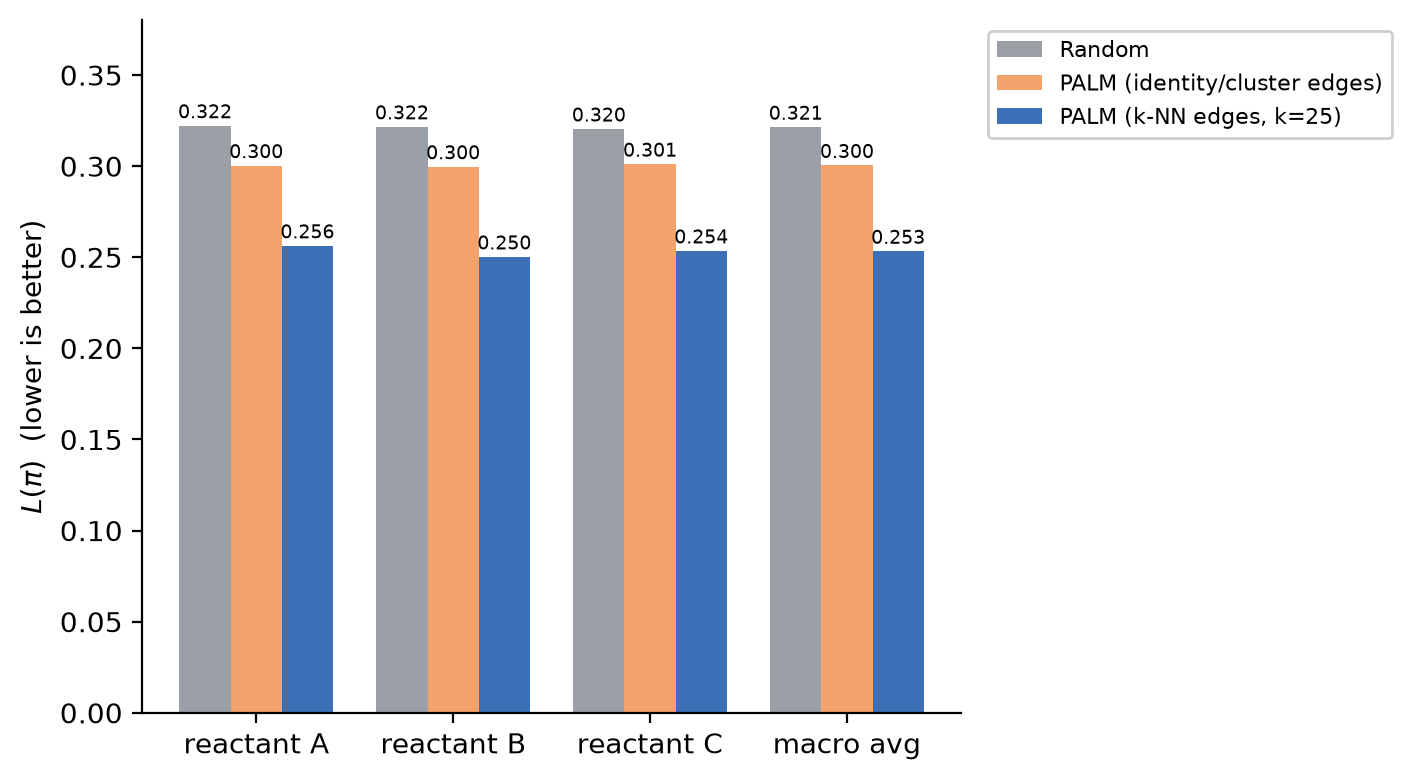
\includegraphics[width=0.78\linewidth]{Figs/mcr_benchmark.png}
    \caption{Per-axis and macro-average leakage (scaled $L(\pi)$, lower is
    better) on the USPTO three-reactant multi-component set ($n=4{,}300$). With
    near-unique reactants, identity/cluster hyperedges (orange) barely improve on
    random (grey); per-axis $k$-NN hyperedges (blue, $k{=}25$) reduce leakage by
    $\sim$$20\%$ on every axis. DataSAIL cannot express this $>2$-axis joint
    split.}
    \label{fig:mcr}
\end{figure}

\begin{figure}[!ht]
    \centering
    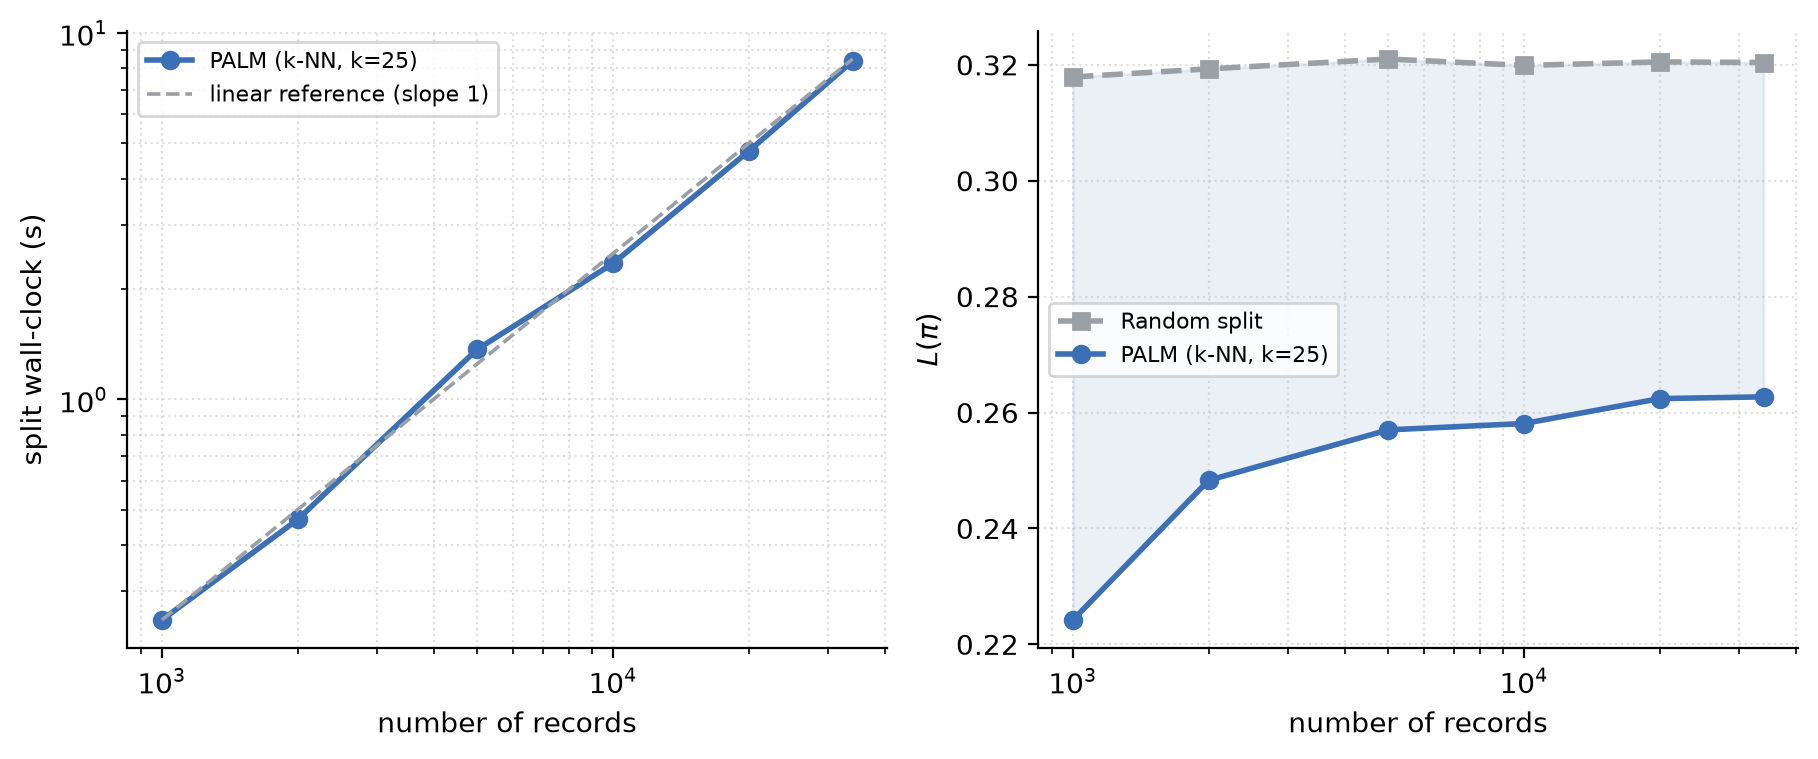
\includegraphics[width=\linewidth]{Figs/mcr_scaling.png}
    \caption{Multi-axis split scaling on the enlarged USPTO multicomponent set (three
    reactant axes, up to $33{,}953$ records). \emph{Left:} split wall-clock vs.\
    number of records (log--log) tracks the unit-slope (linear) reference,
    reaching $33$k records in $8.4$\,s. \emph{Right:} the macro scaled $L(\pi)$
    of the per-axis $k$-NN split ($k{=}25$, blue) stays well below random (grey)
    across two orders of magnitude in $n$. Reported times are the split only;
    one-time Morgan fingerprinting ($4.3$\,s on $48$ cores) is shared across all
    sizes.}
    \label{fig:mcr_scaling}
\end{figure}

\begin{table}[!ht]
  \caption{Multi-axis hypergraph splitting on multi-component reaction datasets
  ($80/20$). Macro scaled $L(\pi)$ averaged over all component axes (lower is
  better). For Buchwald--Hartwig and Suzuki--Miyaura the hypergraph uses identity
  hyperedges (low-cardinality axes); for USPTO-MCR we report both the identity
  and the per-axis $k$-NN ($k{=}25$) construction. DataSAIL is omitted: it
  supports only one- and two-dimensional splits and cannot express a joint split
  over $>2$ axes.}
  \label{tab:reactions}
  \centering
  \small
  \begin{tabular}{lrrccr}
    \toprule
    Dataset & $n$ & Axes & PALM & Random & Time (s) \\
    \midrule
    Buchwald--Hartwig & 3{,}955 & 4 & 0.290 & 0.320 & 0.9 \\
    Suzuki--Miyaura   & 5{,}760 & 5 & 0.314 & 0.321 & 0.1 \\
    USPTO-MCR (identity)        & 4{,}300 & 3 & 0.300          & 0.321 & 0.3 \\
    USPTO-MCR ($k$-NN, $k{=}25$) & 4{,}300 & 3 & \textbf{0.253} & 0.321 & 3.4 \\
    \bottomrule
  \end{tabular}
\end{table}

\begin{ack}
This research was supported by multiple institutional and federal grants. This project is supported by the Eric and Wendy Schmidt AI in Science Postdoctoral Fellowship, a Schmidt Sciences, LLC program. This work was also in part supported by the National Science Foundation Future Manufacturing Project \#2037026. Additional support came from the University of Chicago Data Science Institute through the 2024 AI+Science Research Initiative. We acknowledge the Carbon High-Performance Computing Cluster at the Center for Nanoscale Materials, Argonne National Laboratory, supported by the U.S. Department of Energy Office of Science User Facility under Contract No. DE-AC02-06CH11357. We declare no conflict of interest for this work.
\end{ack}

%\section*{References}
\newpage

\begin{thebibliography}{}

\bibitem{joeres2025}
Joeres, Roman, David B. Blumenthal, and Olga V. Kalinina. ``Data splitting to avoid information leakage with DataSAIL.'' Nature Communications 16.1 (2025): 3337.

\bibitem{joeres2025addendum}
Joeres, Roman, David B. Blumenthal, and Olga V. Kalinina. ``Addendum: Data splitting against information leakage with DataSAIL.'' Nature Communications 17 (2026): 1597.

\bibitem{wu2018moleculenet}
Wu, Zhenqin, et al. ``MoleculeNet: a benchmark for molecular machine learning.'' Chemical Science 9.2 (2018): 513--530.

\bibitem{gottesburen2023}
Gottesb\"uren, Lars, Tobias Heuer, Nikolai Maas, Peter Sanders, and Sebastian Schlag. ``Scalable high-quality hypergraph partitioning.'' ACM Transactions on Algorithms 20.1 (2024): Article 9, 9:1--9:54. (Mt-KaHyPar.)

\bibitem{rogers2010ecfp}
Rogers, David, and Mathew Hahn. ``Extended-connectivity fingerprints.'' Journal of Chemical Information and Modeling 50.5 (2010): 742--754.

\bibitem{kapoor2023leakage}
Kapoor, Sayash, and Arvind Narayanan. ``Leakage and the reproducibility crisis in machine-learning-based science.'' Patterns 4.9 (2023): 100804.

\bibitem{lowe2017uspto}
Lowe, Daniel. ``Chemical reactions from US patents (1976--Sep2016).'' Figshare dataset (2017). doi:10.6084/m9.figshare.5104873. Accessed via the Therapeutics Data Commons (TDC) \texttt{RetroSyn} loader.

\end{thebibliography}


%%%%%%%%%%%%%%%%%%%%%%%%%%%%%%%%%%%%%%%%%%%%%%%%%%%%%%%%%%%%

%%%%%%%%%%%%%%%%%%%%%%%%%%%%%%%%%%%%%%%%%%%%%%%%%%%%%%%%%%%%


\end{document}
